%!TEX program = pdflatex
\documentclass{beamer}

\usepackage{etex}
\reserveinserts{28}

%\useoutertheme[glossy]{wuerzburg}
\useinnertheme[shadow,outline]{chamfered}
%\usecolortheme{shark}
\usecolortheme{beaver}
\beamertemplatenavigationsymbolsempty

\usefonttheme{professionalfonts}
\let\digamma\relax
\usepackage[scale=0.85,stdmathitalics=true,romanfamily=casual]{lucimatx}
\usefonttheme[stillsansseriftext]{serif}

\usepackage{bm}


\usepackage{fancyvrb}



\usepackage{textfit} % commands \scaletoheight{height}{text} and \scaletowidth{width}{text}

\usepackage{tikz}

\usepackage{tcolorbox}

\newtheorem{Alert}{Alert}
\newtheorem{Highlight}{Highlight}

\newcommand{\Species}[1]{{\rmfamily \itshape #1}}
\newcommand{\Real}{\ensuremath{\mathbb{R}}}
\newcommand{\RealN}{\ensuremath{\mathbb{R}^n}}
\newcommand{\RealP}{\ensuremath{\mathbb{R}^p}}
\newcommand{\Mtx}[1]{\ensuremath{\bm{#1}}}
\newcommand{\Inv}[1]{\ensuremath{#1^{-1}}}
\newcommand{\InvMtx}[1]{\ensuremath{\bm{#1}^{-1}}}
\newcommand{\Red}[1]{\textcolor{red}{#1}}
\newcommand{\PsInv}[1]{\ensuremath{\bm{#1}^{+}}}

\usepackage{booktabs}



% --- Macro \xvec
% From a tex.stackexchange.com answer by Todd Lehman
% http://tex.stackexchange.com/questions/44017/dot-notation-for-derivative-of-a-vector
\makeatletter
\newlength\xvec@height%
\newlength\xvec@depth%
\newlength\xvec@width%
\newcommand{\xvec}[2][]{%
  \ifmmode%
    \settoheight{\xvec@height}{$#2$}%
    \settodepth{\xvec@depth}{$#2$}%
    \settowidth{\xvec@width}{$#2$}%
  \else%
    \settoheight{\xvec@height}{#2}%
    \settodepth{\xvec@depth}{#2}%
    \settowidth{\xvec@width}{#2}%
  \fi%
  \def\xvec@arg{#1}%
  \def\xvec@dd{:}%
  \def\xvec@d{.}%
  \raisebox{.2ex}{\raisebox{\xvec@height}{\rlap{%
    \kern.05em%  (Because left edge of drawing is at .05em)
    \begin{tikzpicture}[scale=1]
    \pgfsetroundcap
    \draw (.05em,0)--(\xvec@width-.05em,0);
    \draw (\xvec@width-.05em,0)--(\xvec@width-.15em, .075em);
    \draw (\xvec@width-.05em,0)--(\xvec@width-.15em,-.075em);
    \ifx\xvec@arg\xvec@d%
      \fill(\xvec@width*.45,.5ex) circle (.5pt);%
    \else\ifx\xvec@arg\xvec@dd%
      \fill(\xvec@width*.30,.5ex) circle (.5pt);%
      \fill(\xvec@width*.65,.5ex) circle (.5pt);%
    \fi\fi%
    \end{tikzpicture}%
  }}}%
  #2%
}
\makeatother

% --- Override \vec with an invocation of \xvec.
\let\stdvec\vec
\renewcommand{\vec}[1]{\xvec[]{\bm{#1}}}
% --- Define \dvec and \ddvec for dotted and double-dotted vectors.
\newcommand{\dvec}[1]{\xvec[.]{#1}}
\newcommand{\ddvec}[1]{\xvec[:]{#1}}


\usepackage{pifont}
\newcommand{\weblink}{\ding{43}}  % hand with pointing finger

\definecolor{links}{HTML}{2A1B81}
\hypersetup{colorlinks,linkcolor=,urlcolor=magenta}

\usepackage{tikz}
\usepackage{caption}
\usepackage{subcaption}

\usepackage[inline]{asymptote}
\usepackage{marvosym} % for male/female symbols

\newcommand{\matindex}[1]{\scriptsize#1}% Matrix index

\setbeamersize{description width=2em}
\DeclareMathOperator{\rank}{rank} 
\usepackage{blkarray}





%===========================================================
% Title Info
\title{Scientific Computing for Biologists}
\subtitle{Singular Value Decomposition and Biplots}

\author{Paul M. Magwene}


\date{}

\begin{document}
%===========================================================
\begin{frame}
\titlepage
\end{frame}

%===========================================================
\begin{frame}
  \frametitle{Overview of Lecture}
  
\begin{itemize}
		\item Singular Value Decomposition
		\begin{itemize}
			\item Algebra of SVD
			\item Geometry of SVD
			\item Relationship to Eigendecomposition
			\item Applications of SVD			
		\end{itemize}		
		\item Biplots
		\begin{itemize}
			\item Simultaneous representation of rows and columns of a matrix
		\end{itemize}			
\end{itemize}

\end{frame}
%===========================================================

%===========================================================
\begin{frame}
  \frametitle{Hands-on Session}
\begin{itemize}
    \item SVD and Biplots in R
    \item Applications of SVD in R
    		\begin{itemize}
    		\item `Seriation' using SVD
			  \item Matrix approximation and image compression using SVD
		\end{itemize}
\end{itemize} 


\end{frame}		
%===========================================================


%===========================================================
\begin{frame}[fragile]
  \frametitle{Matrix Decomposition}

\begin{itemize}
\item A ``factorization'' is a re-writing of a mathematical object (number, function, etc.) into the product of other object.

\item Your familiar with factorization as used in arithmetic and algebra.

\begin{align*}
12 &= 3 \times 4 = 2 \times 6  \\
x^2 - 4 &= (x-2)(x+2)
\end{align*}

\end{itemize}




\begin{center}
 \alert{Matrix decomposition is the same idea! A matrix decomposition is a factoring of a matrix into simpler parts.}
\end{center}




\end{frame}
%===========================================================



%===========================================================
\begin{frame}
  \frametitle{Eigendecomposition}


You've already been introduced to one way to decompose a square matrix, $\Mtx{A}$:

$$ \Mtx{A} = \Mtx{V}\Mtx{D}\InvMtx{V} $$

where:
\begin{itemize}
\item  $\Mtx{V}$ is a matrix of eigenvectors (in columns)
\item $\Mtx{D}$ is a diagonal matrix with eigenvalues along diagonal.
\end{itemize}

\medskip
when $\Mtx{A}$ is real-valued and symmetric than $\Mtx{V}$ is orthgonal.

\end{frame}
%===========================================================



%===========================================================
\begin{frame}
  \frametitle{Singular Value Decomposition}

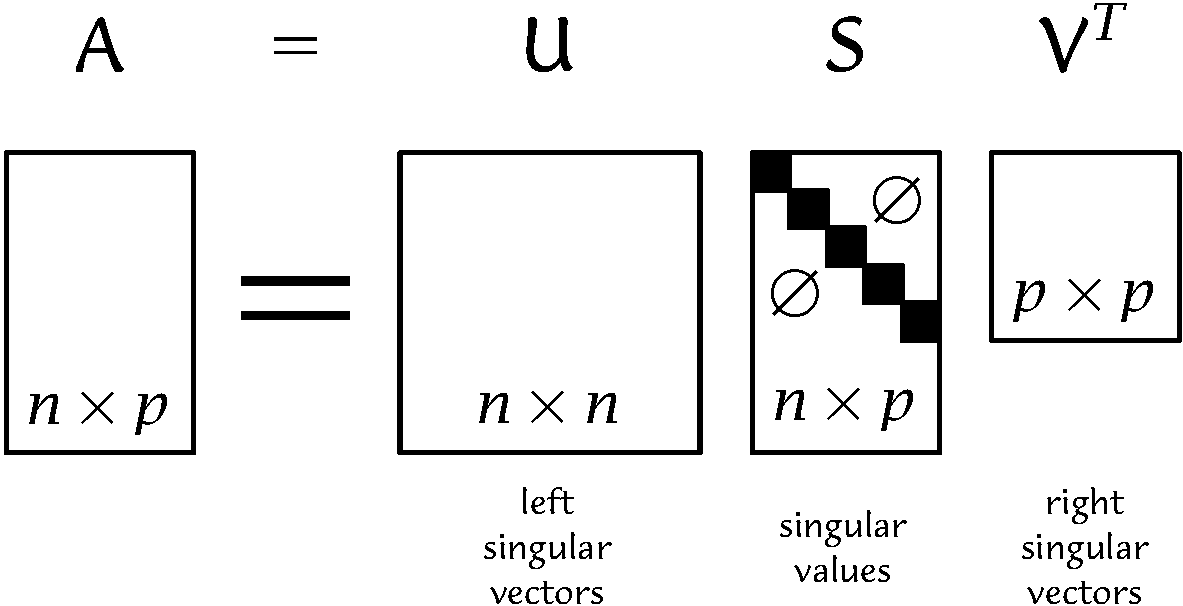
\includegraphics[height=2in]{fig-svd-overview}

\smallskip
\begin{itemize}
  \item When written like this $\Mtx{U}$ and $\Mtx{V}$ are orthonormal.

  \item Sometimes SVD is written as:
\[
\underset{(n \times p)}{\Mtx{A}} = \underset{(n \times p)}{\Mtx{U}} \underset{(p \times p)}{\Mtx{S}} \underset{(p \times p)}{\Mtx{V}^T} 
\]

\end{itemize}


\end{frame}
%===========================================================



%===========================================================
\begin{frame}
  \frametitle{Facts about SVD}

\begin{itemize}
\item Singular Value Decomposition is often referred to as giving the ``basic structure'' of a matrix

\item The rank of $\Mtx{A}$ is equivalent to the number of non-zero singular values in $ \Mtx{A} = \Mtx{U}\Mtx{S}\Mtx{V}^T $

$$ \rank(\Mtx{A}) \leq \min(n,p) $$


\item  The Euclidean norm ($L_2$) norm of a matrix is the relative amount it stretches a vector:

$$ |\Mtx{A}|_E = \frac{|\Mtx{A}\Mtx{x}|}{|\Mtx{x}|} $$

The $L_2$ norm of $\Mtx{A}$ is given by $\Mtx{S}_{11}$.
\end{itemize}



\end{frame}
%===========================================================

%===========================================================
\begin{frame}
  \frametitle{Geometric Interpretation of SVD}

Any matrix, $\Mtx{A}_{n \times p}$, represents a linear transformation from $\RealP \mapsto  \RealN$. 

\medskip
SVD can be thought of decomposing the transformation specified by $\Mtx{A}$ into a simple form:

$$ \Mtx{A} = (\text{rotation})(\text{scaling)}(\text{rotation})$$

\begin{itemize}
\item $\Mtx{U}$ and $\Mtx{V}$ are orthonormal (orthogonal) matrices $\rightsquigarrow$ Orthonormal matrices represent rigid rotations (or rotation plus reflection).
\item Diagonal matrices represent ``stretching''
\end{itemize}


\end{frame}

%===========================================================





%===========================================================
\begin{frame}[fragile]
  \frametitle{SVD Example}

\[
\Mtx{A} =  \begin{bmatrix}3 & 1 \\ 2 & 2\end{bmatrix} = \Mtx{U} \Mtx{S} \Mtx{V}^T
\]
where
\[
\Mtx{U} = \begin{bmatrix} -0.75 & -0.66 \\ -0.66 & 0.75 \end{bmatrix}, \:
\Mtx{S} = \begin{bmatrix} 4.13 & 0 \\ 0 & 0.97 \end{bmatrix}, \:
\Mtx{V}^T = \begin{bmatrix} -0.86 & -0.50 \\ 0.50 & -0.86 \end{bmatrix}
\]

\medskip
\alert{Geometry}
\centerline{
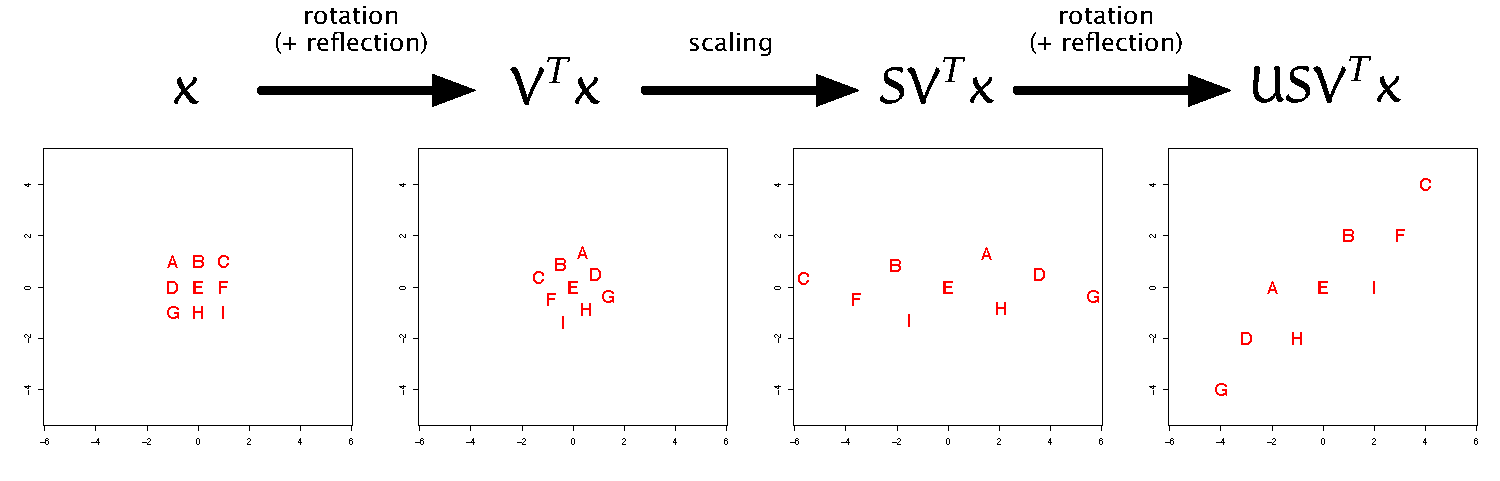
\includegraphics[height=1.5in]{fig-svd-example}
}

\end{frame}
%===========================================================




%===========================================================
\begin{frame}[fragile]
  \frametitle{Relationship of SVD to Eigendecomposition}

\begin{align}
  \Mtx{A} &= \Mtx{U} \Mtx{S} \Mtx{V}^T \\
  \Mtx{A}^ T\Mtx{A} &= (\Mtx{V}\Mtx{S}\Mtx{U}^T)(\Mtx{U} \Mtx{S} \Mtx{V}^T)\\
      &= \Mtx{V} \Mtx{S} \Mtx{U}^T \Mtx{U} \Mtx{S} \Mtx{V}^T \\
      &= \Mtx{V}\Mtx{S}\Mtx{S}\Mtx{V}^T  \label{eq:ortho}
\end{align}
Equation~\ref{eq:ortho} follows from the fact that $\Mtx{U}$ is orthonormal ($\Mtx{U}^T \Mtx{U} = \Mtx{I}$)

\smallskip
If we let $\Mtx{D} = \Mtx{S}\Mtx{S}$, we can rewrite equation~\ref{eq:ortho} as:
\begin{align}
  \Mtx{A}^ T\Mtx{A} &= \Mtx{V}\Mtx{D}\Mtx{V} && \text{\footnotesize Eigendecomposition!}
\end{align}

\begin{itemize}
\item The singular values $\Mtx{S}_{ii}$ are $\sqrt{\Mtx{D}_{ii}}$ where $\Mtx{d}_{ii}$ are the eigenvalues of $\Mtx{A}^ T\Mtx{A}$.

\item The columns of $\Mtx{V}$ are the eigenvectors of $\Mtx{A}^ T\Mtx{A}$.
\end{itemize}

\end{frame}
%===========================================================


%===========================================================
\begin{frame}[fragile]
  \frametitle{Using SVD to do PCA}

Let \Mtx{X} be a mean-centered $n \times p$ data matrix. The covariance matrix is given by:
\begin{align*}
  \Mtx{C} = \tfrac{1}{n-1} \; \Mtx{X}^T \Mtx{X}
\end{align*}

By SVD we can write $\Mtx{X} = \Mtx{U}\Mtx{S}\Mtx{V}^T$, therefore:
\begin{align*}
  \Mtx{C} &= \tfrac{1}{n-1} \; \Mtx{V}\Mtx{S}\Mtx{U}^T \Mtx{U}\Mtx{S}\Mtx{V}^T \\
          &= \tfrac{1}{n-1} \; \Mtx{V} \Mtx{S}\Mtx{S} \Mtx{V}^T
\end{align*}

\begin{itemize}
  \item The PC vectors are given by the columns of \Mtx{V} (rows of $\Mtx{V}^T$)
  \item The PC scores are given by $\Mtx{U}\Mtx{D}$, where $\Mtx{D} = \Mtx{S}\Mtx{S}$
\end{itemize}

\end{frame}
%===========================================================



%===========================================================
\begin{frame}
  \frametitle{Another Way of Thinking about SVD}


\begin{center}
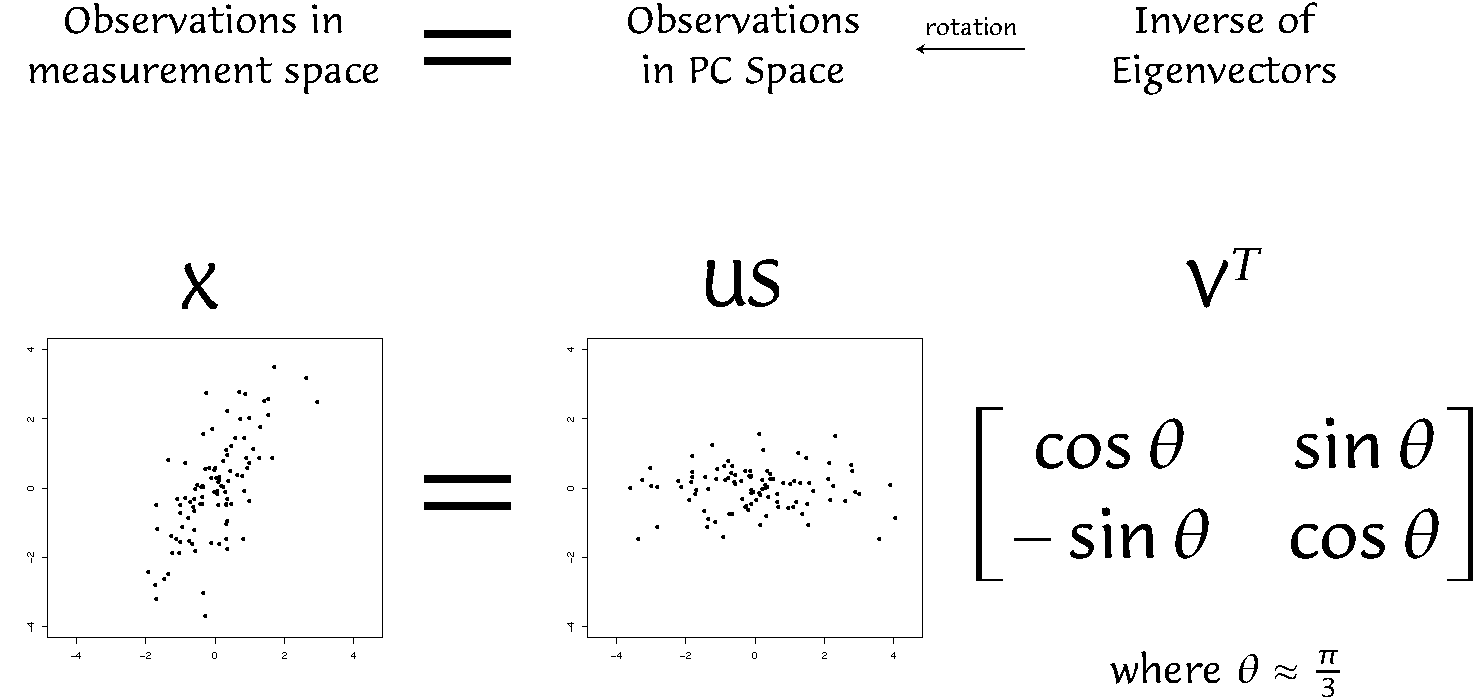
\includegraphics[width=\textwidth]{fig-svdpca}
\end{center}

\end{frame}

%===========================================================


%===========================================================
\begin{frame}
  \frametitle{Applications of SVD}

\begin{itemize}
\item Matrix approximation
\item Efficient PCA
\item Biplots
\item ... and many more ...
\end{itemize}

\end{frame}
%===========================================================


%===========================================================
\begin{frame}
  \frametitle{SVD for Matrix Approximation}

If $ \Mtx{A} = \Mtx{U} \Mtx{S} \Mtx{V}^T $
then the optimal (least-squares) $k$-dimensional approximation of \Mtx{A} (where $ k < \rank(\Mtx{A})$) is given by:
\[
\tilde{\Mtx{A}} = \Mtx{U}\Mtx{S}^{\star} \Mtx{V}^T
\]

where:
\begin{eqnarray*}
\Mtx{S}_{ii}^{\star} &=& \Mtx{S}_{ii} \text{ for } i \leq k\\
\Mtx{S}_{ii}^{\star} &=& 0 \text{ for } i > k\\
\end{eqnarray*}

\end{frame}
%===========================================================



%===========================================================
\begin{frame}
  \frametitle{Biplots}

\begin{itemize}
  \item Technique for simultaneously displaying row and column data (observations and variables)
  \item Invented by K. Gabriel (see also papers by Gower)
\end{itemize}

Given a data matrix, \Mtx{X}, we can use SVD to approximate \Mtx{X} as so:
\begin{gather*}
  \tilde{\Mtx{X}}_k =  \Mtx{U}\Mtx{S}^{\star} \Mtx{V}^T \\
  \text{\footnotesize (k-dimensional approximation to \Mtx{X})}
\end{gather*}


We can rewrite $\tilde{\Mtx{X}}_k$ as a product of two matrices:
\[
  \Mtx{X} = \Mtx{G}\Mtx{H}^T
\]
where
\[
  \Mtx{G} = \Mtx{U}(\Mtx{S}^{\star})^\alpha\; \text{ and } \ \Mtx{H}^T = (\Mtx{S}^{\star})^{1-\alpha}\Mtx{V}^T
\]
\end{frame}

%===========================================================


%===========================================================
\begin{frame}
  \frametitle{Biplots, cont.}

\begin{eqnarray*}
\Mtx{G} &=& \Mtx{U}(\Mtx{S}^{\star})^{\alpha} \text{ (row effects) } \\
\Mtx{H}^T &=& (\Mtx{S}^{\star})^{1-\alpha} \Mtx{V}^T \text{ (columns effects) }
\end{eqnarray*}

Different choices of $\alpha$ emphasize different relationships in the data.

\begin{itemize}
\item \Red{$\alpha = 0$}, column-metric preserving biplot; optimally approximates variance-covariance structure. Cosine of angles between vectors approximate correlations; distances between points approximate Mahalanobis distance ( ``correlation biplot'')
\item \Red{$\alpha = 1$}, row-metric preserving biplot; optimally approximates Euclidean distances among observations. Coordinates of observations correspond to PC scores; coordinates of variables correspond to eigenvector coefficients (``distance biplot''). PCs are `sphered'.
% \item \Red{$\alpha = 0.5$},  optimally approximates observational values (``symmetric biplot'')
\end{itemize}

\end{frame}

%===========================================================

%===========================================================
\begin{frame}
  \frametitle{Biplots, Example}

\begin{itemize}
\item Observations drawn as points in space of PCs
\item Variables drawn as vectors in PC space
\end{itemize}

\medskip

\centerline{
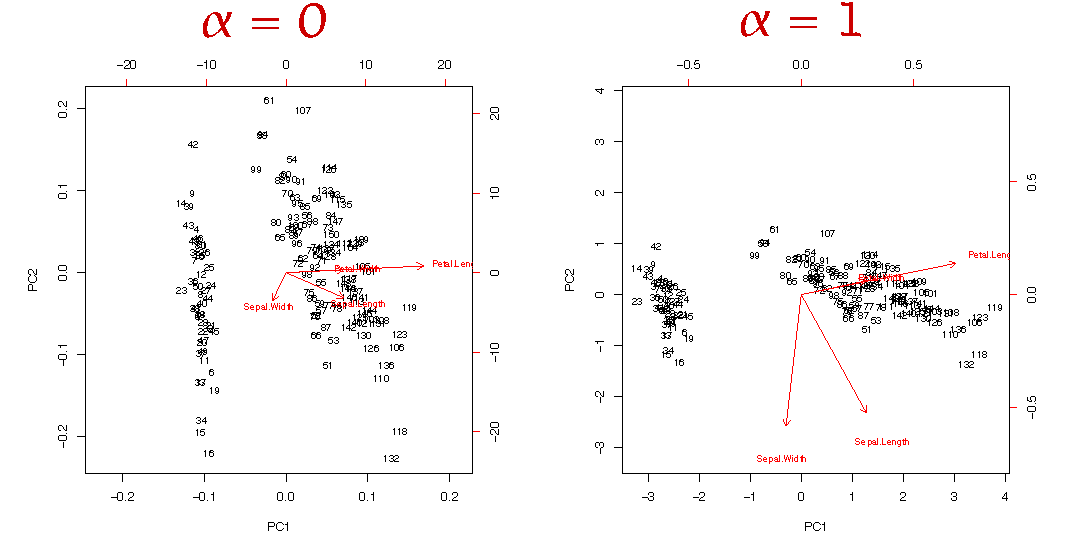
\includegraphics[height=1.9in]{fig-irisbiplot-simple.pdf}
}
\begin{center}
PCA Biplots of Iris data set.
\end{center}

\end{frame}

%===========================================================


\end{document}


%===========================================================
\begin{frame}
  \frametitle{XXX}

\end{frame}
%===========================================================
